
\newpage



\FloatBarrier

\appendix

\begin{center}
{\LARGE{Appendix}}

{``Applying Data Synthesis for Longitudinal Business Data across Three Countries''}

\textit{M. Jahangir Alam, Benoit Dostie, J\"org Drechsler, Lars Vilhuber}

\end{center}


\section{Figures for the Manufacturing Sector in Canada}
\label{sec:appendix_figures}

\begin{figure}[H]
\centering
\begin{subfigure}[h]{0.48\linewidth}
\label{tab:Can:GrossEmploymentPrivate}
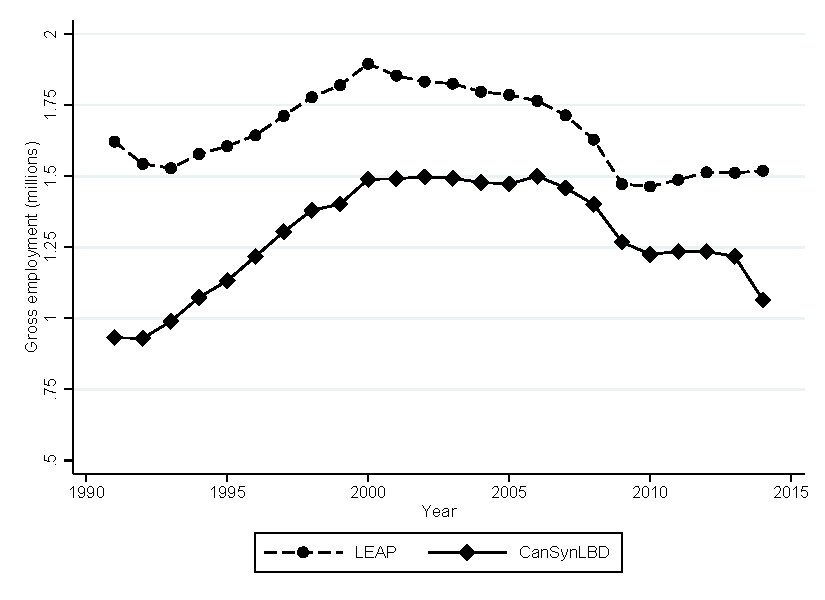
\includegraphics[width=\linewidth]{graphs/Gross_employment_level_by_year_manufacturing_bw.pdf} 
\caption{Gross employment level by year} \end{subfigure}
\hfill
\begin{subfigure}[h]{0.48\linewidth}
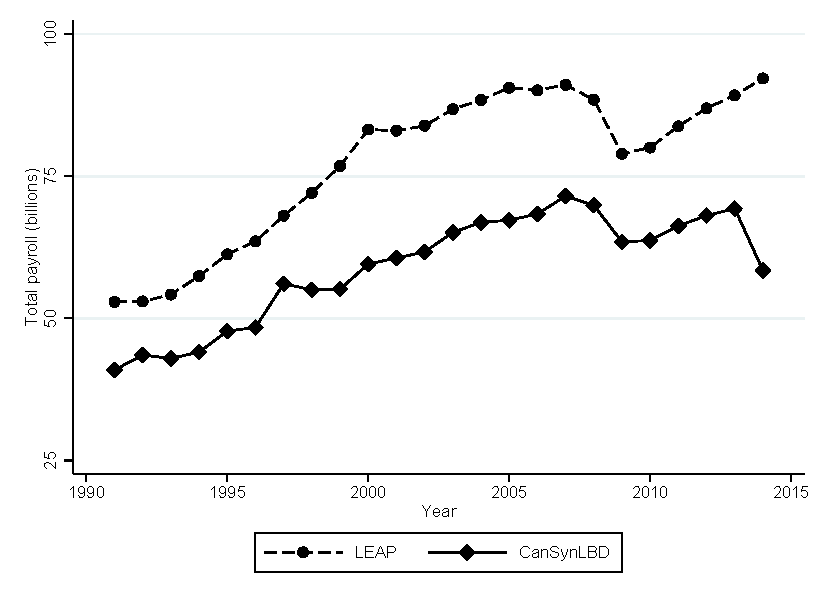
\includegraphics[width=\linewidth]{graphs/Total_payroll_by_year_manufacturing_bw.pdf}
\caption{Total payroll}
\end{subfigure}\caption{Entity characteristics for the manufacturing sector in Canada by year.}\label{fig:entity_chracteristics_manufac}
\end{figure}


\begin{figure}[H]
\begin{subfigure}[h]{0.48\linewidth}
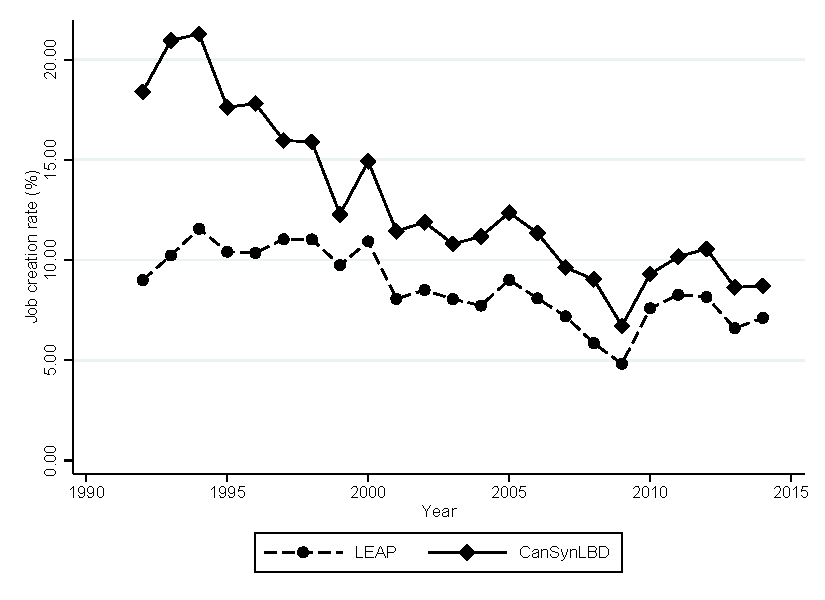
\includegraphics[width=\linewidth]{graphs/Job_creation_rate_by_year_Manufacturing_bw.pdf}
\caption{Job creation rates}
\end{subfigure}
\hfill
\begin{subfigure}[h]{0.48\linewidth}
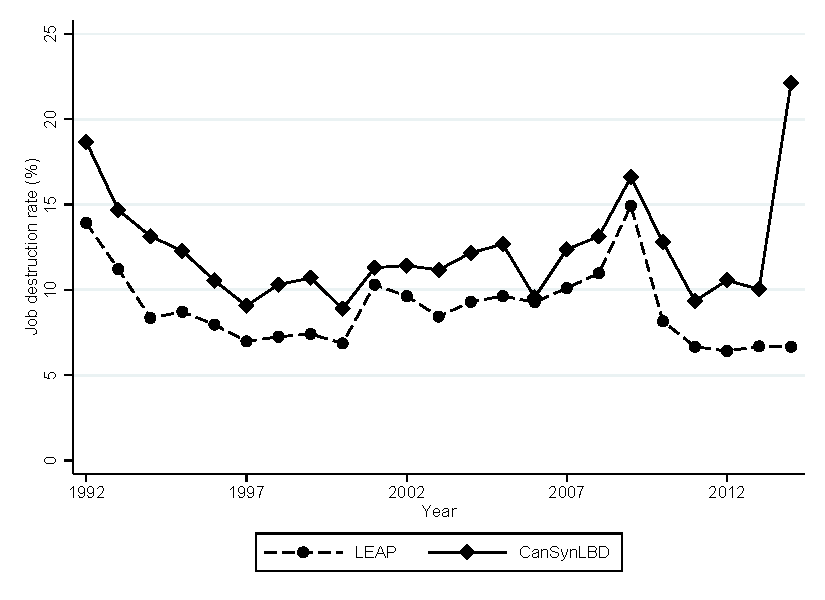
\includegraphics[width=\linewidth]{graphs/Job_destruction_rate_by_year_Manufacturing_bw.pdf}
\caption{Job destruction rates}
\end{subfigure}\caption{Dynamics of job flows for the manufacturing sector in Canada by year.}\label{fig:job_flows_manufac}
\end{figure}





















\begin{figure}[H]
\centering
\begin{subfigure}[h]{0.5\linewidth}
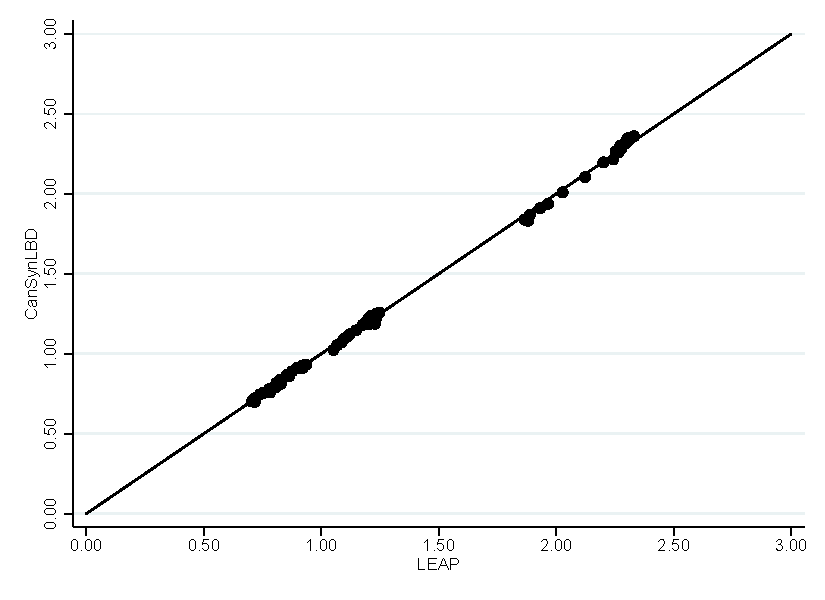
\includegraphics[trim=0 10 0 0,clip, width=\linewidth]{graphs/Share_of_firms_by_NAICS_two-digit_and_year_Manufacturing_bw.pdf}
\end{subfigure}\\
\begin{subfigure}[h]{0.5\linewidth}
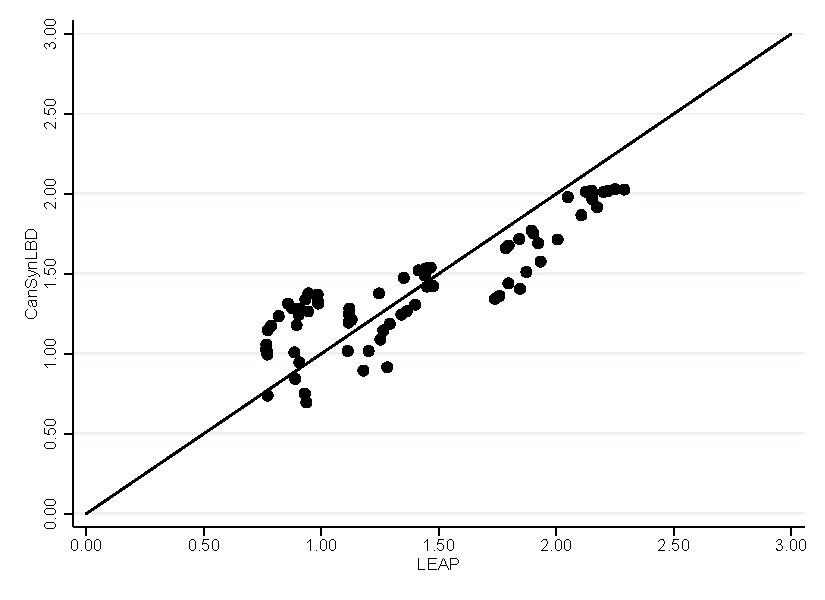
\includegraphics[trim=0 10 0 -20,clip,width=\linewidth]{graphs/Share_of_employment_by_NAICS_two-digit_and_year_Manufacturing_bw.pdf}
\end{subfigure}\\
\begin{subfigure}[h]{0.5\linewidth}
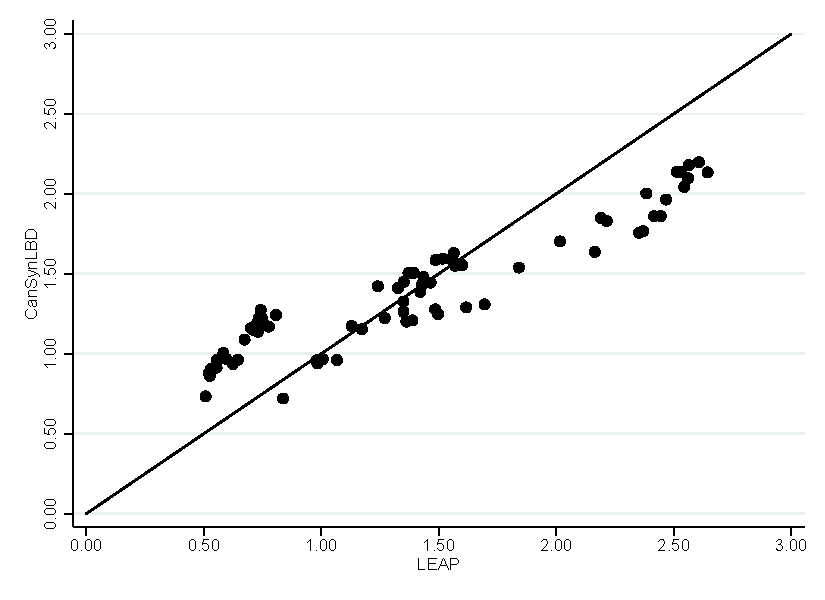
\includegraphics[trim=0 0 0 -20,clip,width=\linewidth]{graphs/Share_of_payroll_by_NAICS_two-digit_and_year_Manufacturing_bw.pdf}
\end{subfigure}
\caption{Share of entities (upper panel), share of employment (middle panel), and share of payroll (lower panel) by year and industry for the Canadian manufacturing sector.}\label{fig:FirmShare_manufac}
\end{figure}


































\FloatBarrier
\clearpage

\section{Appendix Tables}
\label{sec:appendix_tables}






\subsection{pMSE}
\label{sec:pmse_tables}










\begin{table}[!htbp] \centering 
\setlength{\tabcolsep}{11pt}
\begin{threeparttable}
  \caption{Detailed results for pMSE estimation by sector and country} 
  \label{tab:pmse:details} 
\begin{tabular}{@{\extracolsep{5pt}} l|cc|c} 
\toprule
\textbf{Independent Variables} & \multicolumn{2}{c|}{\textbf{Canada}} & \textbf{Germany}\\
\multicolumn{1}{r|}{\it Sector:}&Manufacturing & Private & All \\ 
\midrule
Ln ALU & 0.158 & 0.7138 & -0.2895 \\ 
 & (0.0039) & (0.001) & (0.0033)\\
Ln Pay & 0.0039 & -0.4426 & 0.2584 \\ 
 & (0.0037) & (0.001) & (0.0028)\\
Age 3-4 & 0.0392 & 0.0972 & -0.0987 \\ 
 & (0.0078) & (0.0017) & (0.007)\\ 
Age 5-7 & -0.0382 & 0.0477 & -0.0973 \\ 
 & (0.0073) & (0.0016) & (0.0066)\\ 
Age 8-12 & -0.1258 & -0.0263 & -0.1172 \\ 
 & (0.0071) & (0.0015) & (0.0063)\\ 
Age 13 or more & -0.219 & -0.1024 & -0.1487 \\ 
 & (0.0074) & (0.0016) & (0.0059)\\ 
 \midrule
N & 2243011 & 34638723 & 2121956 \\ 
pseudo R-sq & 0.0112 & 0.0318 & 0.0038 \\ 
\midrule
pMSE & 0.0041 & 0.0121 & 0.0013 \\ 
\bottomrule
\end{tabular} 
\begin{tablenotes}
\small
\item \textit{Note}: See Equation~\ref{pMSE} for estimation method. An observation is a entity-year in the combined database of each country-sector combination. All specifications include  time and industry fixed effects. Standard errors are in parentheses. 
\end{tablenotes}
\end{threeparttable}
\end{table} 

\clearpage
\FloatBarrier
\clearpage
 
\subsection{Regression analysis tables}
\label{sec:regression_tables}

\begin{table}[H]
  \centering
\begin{threeparttable}
 \caption{Regression coefficients (OLS) for LEAP} \label{tab:OLS_can} \medskip
\renewcommand{\arraystretch}{1}
\begin{tabular}{l|c c| c c}
\toprule
\textbf{Independent Variables}&\multicolumn{2}{c|}{\textbf{LEAP}} &  \multicolumn{2}{c}{\textbf{CanSynLBD}}\\
\midrule
&\multicolumn{1}{c}{Private}&\multicolumn{1}{c}{Manufacturing}&\multicolumn{1}{c}{Private}&\multicolumn{1}{c}{Manufacturing}\\
\hline
AR(1) Coefficient&   0.2031\sym{***}&   0.2481\sym{***}&   0.3970\sym{***}&   0.4405\sym{***}\\
          & (0.0001)         & (0.0005)         & (0.0002)         & (0.0007)         \\
[1em]
Ln Pay    &   0.7847\sym{***}&   0.7300\sym{***}&   0.5481\sym{***}&   0.5228\sym{***}\\
          & (0.0001)         & (0.0005)         & (0.0002)         & (0.0006)         \\
[1em]
Age 3-4   &  -0.1202\sym{***}&  -0.1717\sym{***}&  -0.1223\sym{***}&  -0.2340\sym{***}\\
          & (0.0003)         & (0.0014)         & (0.0004)         & (0.0016)         \\
[1em]
Age 5-7   &  -0.1260\sym{***}&  -0.1891\sym{***}&  -0.1235\sym{***}&  -0.2507\sym{***}\\
          & (0.0003)         & (0.0014)         & (0.0004)         & (0.0016)         \\
[1em]
Age 8-12  &  -0.1268\sym{***}&  -0.1973\sym{***}&  -0.1169\sym{***}&  -0.2551\sym{***}\\
          & (0.0003)         & (0.0013)         & (0.0004)         & (0.0016)         \\
[1em]
Age 13 or more&  -0.1246\sym{***}&  -0.1992\sym{***}&  -0.1101\sym{***}&  -0.2577\sym{***}\\
          & (0.0003)         & (0.0014)         & (0.0004)         & (0.0017)         \\
\hline
\(N\)     & 15708195         &  1015293         & 13573225         &   959764         \\
\(R^{2}\) &   0.9696         &   0.9743         &   0.9444         &   0.9523         \\
 \bottomrule
\end{tabular} 
\begin{tablenotes}
\small
\item Note: In all specifications, we include both year and industry fixed effects. Standard errors are in parentheses.  ***, **, and * indicate statistically significant coefficients at 1\%, 5\%, and 10\% percent levels, respectively.
 \end{tablenotes}
 \end{threeparttable}
\end{table}

\begin{table}[H]
  \centering
\caption{Regression coefficients (OLS) for GLBD} \label{tab:OLS_ger} \medskip
\renewcommand{\arraystretch}{1}
\setlength{\tabcolsep}{14pt}
\begin{tabular}{l|c |c}
\toprule
\textbf{Independent Variables}&\textbf{GLBD} &  \textbf{GSynLBD}\\
\midrule

AR(1) Coefficient&   0.4430\sym{***}&   0.4143\sym{***}\\
          & (0.0007)         & (0.0008)         \\
[1em]
Ln Pay    &   0.4629\sym{***}&   0.5143\sym{***}\\
          & (0.0006)         & (0.0007)         \\
[1em]
Age 3-4   &  -0.0695\sym{***}&  -0.0642\sym{***}\\
          & (0.0017)         & (0.0016)         \\
[1em]
Age 5-7   &  -0.1066\sym{***}&  -0.0891\sym{***}\\
          & (0.0017)         & (0.0016)         \\
[1em]
Age 8-12  &  -0.1324\sym{***}&  -0.1109\sym{***}\\
          & (0.0017)         & (0.0016)         \\
[1em]
Age 13 or more&  -0.1880\sym{***}&  -0.1600\sym{***}\\
          & (0.0016)         & (0.0015)         \\
\midrule
\(N\)     &   848871         &   966084         \\
\(R^{2}\) &   0.9167         &   0.8968         \\
    \bottomrule
  \end{tabular} 
\begin{tablenotes}
\small
\item Note: In all specifications, we include both year and industry fixed effects. Standard errors are in parentheses.  ***, **, and * indicate statistically significant coefficients at 1\%, 5\%, and 10\% percent levels, respectively.
 \end{tablenotes}
\end{table}




\begin{table}[H]
  \centering
\begin{threeparttable}
 \caption{Regression coefficients (Dynamic) for LEAP} \label{tab:Dynamic - GMM_can} \medskip
\renewcommand{\arraystretch}{1}
\begin{tabular}{l|c c| c c}
\toprule
\textbf{Independent Variables}&\multicolumn{2}{c|}{\textbf{LEAP}} &  \multicolumn{2}{c}{\textbf{CanSynLBD}}\\
\midrule
&\multicolumn{1}{c}{Private}&\multicolumn{1}{c}{Manufacturing}&\multicolumn{1}{c}{Private}&\multicolumn{1}{c}{Manufacturing}\\
\hline
AR(1) Coefficient&   0.0805\sym{***}&   0.1189\sym{***}&   0.5722\sym{***}&   0.5425\sym{***}\\
          & (0.0003)         & (0.0018)         & (0.0024)         & (0.0084)         \\
[1em]
Ln Pay    &   0.8991\sym{***}&   0.8523\sym{***}&   0.4101\sym{***}&   0.4302\sym{***}\\
          & (0.0002)         & (0.0015)         & (0.0018)         & (0.0067)         \\
[1em]
Age 3-4   &  -0.0450\sym{***}&  -0.0797\sym{***}&  -0.2075\sym{***}&  -0.2972\sym{***}\\
          & (0.0002)         & (0.0014)         & (0.0010)         & (0.0051)         \\
[1em]
Age 5-7   &  -0.0438\sym{***}&  -0.0860\sym{***}&  -0.2129\sym{***}&  -0.3162\sym{***}\\
          & (0.0002)         & (0.0015)         & (0.0011)         & (0.0059)         \\
[1em]
Age 8-12  &  -0.0418\sym{***}&  -0.0923\sym{***}&  -0.2187\sym{***}&  -0.3294\sym{***}\\
          & (0.0003)         & (0.0017)         & (0.0013)         & (0.0070)         \\
[1em]
Age 13 or more&  -0.0379\sym{***}&  -0.0898\sym{***}&  -0.2318\sym{***}&  -0.3414\sym{***}\\
          & (0.0003)         & (0.0019)         & (0.0015)         & (0.0080)         \\
\hline
\(N\)     & 15708195         &  1015293         & 13573225         &   959764         \\
m2        & -14.5000         &  -2.2200         & -27.5400         &  -9.4400         \\
Sargan test&  6.9e+04         &  4.6e+03         &  1.5e+04         &  1.5e+03         \\
df of Sargan Test& 252.0000         & 252.0000         & 252.0000         & 252.0000         \\
P value of Sargan test&   0.0000         &   0.0000         &   0.0000         &   0.0000         \\
    \bottomrule
  \end{tabular} 
\begin{tablenotes}
\small
\item Note: In this table, $m2$ is the Arellano-Bond test for zero autocorrelation in first-differenced errors for order two. Standard errors are in parentheses. ***, **, and * indicate statistically significant coefficients at 1\%, 5\%, and 10\% percent levels, respectively.
 \end{tablenotes}
 \end{threeparttable}
\end{table}

\begin{table}[H]
  \centering
\caption{Regression coefficients (Dynamic) for GLBD} \label{tab:Dynamic - GMM_ger} \medskip
\renewcommand{\arraystretch}{1}
\setlength{\tabcolsep}{13pt}
\begin{tabular}{l|c |c}
\toprule
\textbf{Independent Variables}&\textbf{GLBD} &\textbf{GSynLBD}\\
\midrule
AR(1) Coefficient&   0.0489\sym{***}&   0.6999\sym{***}\\
          & (0.0051)         & (0.0057)         \\
[1em]
Ln Pay    &   0.7559\sym{***}&   0.2916\sym{***}\\
          & (0.0035)         & (0.0042)         \\
[1em]
Age 3-4   &  -0.0070\sym{***}&  -0.1026\sym{***}\\
          & (0.0012)         & (0.0015)         \\
[1em]
Age 5-7   &  -0.0233\sym{***}&  -0.1386\sym{***}\\
          & (0.0014)         & (0.0017)         \\
[1em]
Age 8-12  &  -0.0473\sym{***}&  -0.1694\sym{***}\\
          & (0.0015)         & (0.0018)         \\
[1em]
Age 13 or more&  -0.1084\sym{***}&  -0.2183\sym{***}\\
          & (0.0015)         & (0.0018)         \\
\hline
\(N\)     &   848871         &   966084         \\
m2        &  -2.5100         &  -4.1300         \\
Sargan test&  3.6e+03         &  2.0e+03         \\
df of Sargan Test& 495.0000         & 495.0000         \\
P value of Sargan test&   0.0000         &   0.0000         \\
    \bottomrule
  \end{tabular} 
\begin{tablenotes}
\small
\item Note: In this table, $m2$ is the Arellano-Bond test for zero autocorrelation in first-differenced errors for order two. Standard errors are in parentheses. ***, **, and * indicate statistically significant coefficients at 1\%, 5\%, and 10\% percent levels, respectively.
 \end{tablenotes}
\end{table}





\begin{table}[H]
  \centering
\begin{threeparttable}
 \caption{Regression coefficients (Dynamic - system GMM) for LEAP} \label{tab:Dynamic - system GMM_can} \medskip
\renewcommand{\arraystretch}{1}
\begin{tabular}{l|c c| c c}
\toprule
\textbf{Independent Variables}&\multicolumn{2}{c|}{\textbf{LEAP}} &  \multicolumn{2}{c}{\textbf{CanSynLBD}}\\
\midrule
&\multicolumn{1}{c}{Private}&\multicolumn{1}{c}{Manufacturing}&\multicolumn{1}{c}{Private}&\multicolumn{1}{c}{Manufacturing}\\
\hline
AR(1) Coefficient&   0.0978\sym{***}&   0.1614\sym{***}&   0.5111\sym{***}&   0.5780\sym{***}\\
          & (0.0002)         & (0.0014)         & (0.0008)         & (0.0041)         \\
[1em]
Ln Pay    &   0.8854\sym{***}&   0.8161\sym{***}&   0.4562\sym{***}&   0.4022\sym{***}\\
          & (0.0002)         & (0.0012)         & (0.0006)         & (0.0033)         \\
[1em]
Age 3-4   &  -0.0555\sym{***}&  -0.1097\sym{***}&  -0.1828\sym{***}&  -0.3177\sym{***}\\
          & (0.0002)         & (0.0012)         & (0.0004)         & (0.0028)         \\
[1em]
Age 5-7   &  -0.0558\sym{***}&  -0.1201\sym{***}&  -0.1860\sym{***}&  -0.3408\sym{***}\\
          & (0.0002)         & (0.0013)         & (0.0005)         & (0.0031)         \\
[1em]
Age 8-12  &  -0.0548\sym{***}&  -0.1298\sym{***}&  -0.1875\sym{***}&  -0.3583\sym{***}\\
          & (0.0002)         & (0.0014)         & (0.0005)         & (0.0036)         \\
[1em]
Age 13 or more&  -0.0524\sym{***}&  -0.1317\sym{***}&  -0.1943\sym{***}&  -0.3747\sym{***}\\
          & (0.0002)         & (0.0016)         & (0.0006)         & (0.0041)         \\
\hline
\(N\)     & 15708195         &  1015293         & 13573225         &   959764         \\
m2        & -11.4300         &   1.3900         & -41.6000         &  -7.6700         \\
Sargan test&  7.7e+04         &  6.3e+03         &  1.8e+04         &  1.7e+03         \\
df of Sargan Test& 274.0000         & 274.0000         & 274.0000         & 274.0000         \\
P value of Sargan test&   0.0000         &   0.0000         &   0.0000         &   0.0000         \\
    \bottomrule
  \end{tabular} 
\begin{tablenotes}
\small
\item Note: An observation is an entity-year. In this table, $m2$ is the Arellano-Bond test for zero autocorrelation in first-differenced errors for order two. Standard errors are in parentheses. ***, **, and * indicate statistically significant coefficients at 1\%, 5\%, and 10\% percent levels, respectively.
 \end{tablenotes}
 \end{threeparttable}
\end{table}

\begin{table}[H]
  \centering
\caption{Regression coefficients (Dynamic - system GMM) for GLBD} \label{tab:Dynamic - system GMM_ger} \medskip
\renewcommand{\arraystretch}{1}
\setlength{\tabcolsep}{14pt}
\begin{tabular}{l|c| c}
\toprule
\textbf{Independent Variables}&\textbf{GLBD} &\textbf{GSynLBD}\\
\midrule
AR(1) Coefficient&   0.1883\sym{***}&   0.6140\sym{***}\\
          & (0.0021)         & (0.0027)         \\
[1em]
Ln Pay    &   0.6599\sym{***}&   0.3553\sym{***}\\
          & (0.0014)         & (0.0020)         \\
[1em]
Age 3-4   &  -0.0292\sym{***}&  -0.0934\sym{***}\\
          & (0.0011)         & (0.0013)         \\
[1em]
Age 5-7   &  -0.0512\sym{***}&  -0.1266\sym{***}\\
          & (0.0011)         & (0.0014)         \\
[1em]
Age 8-12  &  -0.0791\sym{***}&  -0.1545\sym{***}\\
          & (0.0011)         & (0.0015)         \\
[1em]
Age 13 or more&  -0.1400\sym{***}&  -0.2012\sym{***}\\
          & (0.0011)         & (0.0015)         \\
\hline
\(N\)     &   848871         &   966084         \\
m2        &  19.4900         &  -8.8300         \\
Sargan test&  4.5e+03         &  2.8e+03         \\
df of Sargan Test& 526.0000         & 526.0000         \\
P value of Sargan test&   0.0000         &   0.0000         \\
    \bottomrule
  \end{tabular} 
\begin{tablenotes}
\small
\item Note: An observation is an entity-year. In this table, $m2$ is the Arellano-Bond test for zero autocorrelation in first-differenced errors for order two. Standard errors are in parentheses. ***, **, and * indicate statistically significant coefficients at 1\%, 5\%, and 10\% percent levels, respectively.
 \end{tablenotes}
\end{table}










\begin{table}[H]
  \centering
\begin{threeparttable}
 \caption{Regression coefficients (Dynamic - system GMM with MA(1)) for LEAP} \label{tab:Dynamic - system GMM with MA(1)_can} \medskip
\renewcommand{\arraystretch}{1}
\begin{tabular}{l|c c| c c}
\toprule
\textbf{Independent Variables}&\multicolumn{2}{c|}{\textbf{LEAP}} &  \multicolumn{2}{c}{\textbf{CanSynLBD}}\\
\midrule
&\multicolumn{1}{c}{Private}&\multicolumn{1}{c}{Manufacturing}&\multicolumn{1}{c}{Private}&\multicolumn{1}{c}{Manufacturing}\\
\hline
AR(1) Coefficient&   0.2005\sym{***}&   0.2821\sym{***}&   0.4850\sym{***}&   0.5737\sym{***}\\
          & (0.0007)         & (0.0040)         & (0.0012)         & (0.0059)         \\
[1em]
Ln Pay    &   0.8044\sym{***}&   0.7135\sym{***}&   0.4760\sym{***}&   0.4056\sym{***}\\
          & (0.0005)         & (0.0034)         & (0.0009)         & (0.0046)         \\
[1em]
Age 3-4   &  -0.1245\sym{***}&  -0.2033\sym{***}&  -0.1716\sym{***}&  -0.3158\sym{***}\\
          & (0.0005)         & (0.0032)         & (0.0006)         & (0.0037)         \\
[1em]
Age 5-7   &  -0.1328\sym{***}&  -0.2264\sym{***}&  -0.1733\sym{***}&  -0.3389\sym{***}\\
          & (0.0005)         & (0.0035)         & (0.0006)         & (0.0043)         \\
[1em]
Age 8-12  &  -0.1383\sym{***}&  -0.2454\sym{***}&  -0.1731\sym{***}&  -0.3560\sym{***}\\
          & (0.0006)         & (0.0039)         & (0.0007)         & (0.0051)         \\
[1em]
Age 13 or more&  -0.1441\sym{***}&  -0.2586\sym{***}&  -0.1774\sym{***}&  -0.3717\sym{***}\\
          & (0.0006)         & (0.0042)         & (0.0008)         & (0.0058)         \\
\hline
\(N\)     & 15708195         &  1015293         & 13573225         &   959764         \\
m2        &   8.2000         &   7.0600         & -40.0300         &  -6.6400         \\
Sargan test&  2.8e+04         &  2.3e+03         &  1.7e+04         &  1.3e+03         \\
df of Sargan Test& 251.0000         & 251.0000         & 251.0000         & 251.0000         \\
P value of Sargan test&   0.0000         &   0.0000         &   0.0000         &   0.0000         \\
    \bottomrule
  \end{tabular} 
\begin{tablenotes}
\small
\item Note: An observation is a firm and a year. In this table, $m2$ is the Arellano-Bond test for zero autocorrelation in first-differenced errors for order two.  Standard errors are in parentheses. ***, **, and * indicate statistically significant coefficients at 1\%, 5\%, and 10\% percent levels, respectively.
 \end{tablenotes}
 \end{threeparttable}
\end{table}

\begin{table}[H]
  \centering
\caption{Regression coefficients (Dynamic - system GMM with MA(1)) for GLBD} \label{tab:Dynamic - system GMM with MA(1)_ger} \medskip
\renewcommand{\arraystretch}{1}
\setlength{\tabcolsep}{14pt}
\begin{tabular}{l|c| c}
\toprule
\textbf{Independent Variables}&\textbf{GLBD} &\textbf{GSynLBD}\\
\midrule
AR(1) Coefficient&   0.3701\sym{***}&   0.5268\sym{***}\\
          & (0.0060)         & (0.0048)         \\
[1em]
Ln Pay    &   0.5349\sym{***}&   0.4202\sym{***}\\
          & (0.0041)         & (0.0036)         \\
[1em]
Age 3-4   &  -0.0594\sym{***}&  -0.0831\sym{***}\\
          & (0.0015)         & (0.0013)         \\
[1em]
Age 5-7   &  -0.0922\sym{***}&  -0.1105\sym{***}\\
          & (0.0018)         & (0.0015)         \\
[1em]
Age 8-12  &  -0.1252\sym{***}&  -0.1351\sym{***}\\
          & (0.0019)         & (0.0016)         \\
[1em]
Age 13 or more&  -0.1850\sym{***}&  -0.1802\sym{***}\\
          & (0.0019)         & (0.0017)         \\
\hline
\(N\)     &   848871         &   966084         \\
m2        &  19.0300         & -11.6900         \\
Sargan test&  3.1e+03         &  2.5e+03         \\
df of Sargan Test& 494.0000         & 494.0000         \\
P value of Sargan test&   0.0000         &   0.0000         \\
    \bottomrule
  \end{tabular} 
\begin{tablenotes}
\small
\item Note: An observation is a firm and a year. In this table, $m2$ is the Arellano-Bond test for zero autocorrelation in first-differenced errors for order two. Standard errors are in parentheses. ***, **, and * indicate statistically significant coefficients at 1\%, 5\%, and 10\% percent levels, respectively.
 \end{tablenotes}
\end{table}
















\section{Canada: Synthesized Observations}
\label{sec:synth_obs}


\begin{table}[H]
  \centering
\begin{threeparttable}
  \caption{Synthesized observations}  \label{tab:Synthesized_observations} \medskip
  \renewcommand{\arraystretch}{1}
  \begin{tabular}{l  c c }
    \toprule
    \textbf{Category}&\textbf{\# of Observations (millions)}&\textbf{Percentage}\\
    \midrule
Synthesized&22.01&93.35\\
Not synthesized&1.57&6.65\\
Total&23.58&100.00\\
    \bottomrule
  \end{tabular} 
\begin{tablenotes}
\small
\item Note: Industries that are not synthesized are NAICS 4481,    4482,     4483,     4511,     4513,     4841,     4842, 5241, and 5242. We drop observations from  synthesized industries when there are  less than ten observations in a given year. We do not synthesize the public sector (NAICS 61, 62, and 91).
 \end{tablenotes}
 \end{threeparttable}
\end{table}
 
\section{Confidentiality assessment}
\label{sec:conf:appendix}


\begin{table}[H]
\centering\footnotesize
\caption{Observed entity births given synthetic births for LEAP.} \label{tab:Can:ProbabilityPrivate} \medskip
\renewcommand{\arraystretch}{1}
\begin{tabular}{c c| c c c}
\toprule
\multicolumn{2}{c|}{\textbf{First (Birth) Year}} &  \multicolumn{3}{c}{\textbf{\% of Births over NAICS}}\\
\textbf{Synthetic}&\textbf{Actual}&\textbf{Minimum}&\textbf{Mean}&\textbf{Maximum}\\
\midrule
1991&1991&0.00&27.69&83.02\\
1992&1992&0.00&3.37&11.11\\
1993&1993&0.00&3.79&33.33\\
1994&1994&0.00&3.73&33.33\\
1995&1995&0.00&3.86&20.00\\
1996&1996&0.00&4.25&33.33\\
1997&1997&0.00&4.10&16.94\\
1998&1998&0.00&4.41&25.00\\
1999&1999&0.00&4.23&33.33\\
2000&2000&0.00&3.41&25.00\\
2001&2001&0.00&2.73&22.22\\
2002&2002&0.00&2.65&25.00\\
2003&2003&0.00&2.22&10.00\\
2004&2004&0.00&2.60&17.86\\
2005&2005&0.00&2.71&20.00\\
2006&2006&0.00&2.83&50.00\\
2007&2007&0.00&2.90&33.33\\
2008&2008&0.00&2.38&20.00\\
2009&2009&0.00&2.47&50.00\\
2010&2010&0.00&2.12&33.33\\
2011&2011&0.00&2.65&50.00\\
2012&2012&0.00&2.41&20.00\\
2013&2013&0.00&2.48&25.00\\
2014&2014&0.00&2.23&20.00\\
2015&2015&0.00&2.15&33.33\\
 \bottomrule
\end{tabular} 
\\
\justify
\end{table}
 

\begin{table}[H]
\centering\footnotesize
\caption{Observed entity births given synthetic births (GLBD)} \label{tab:GLBD:Probability} \medskip
\renewcommand{\arraystretch}{1}
\begin{tabular}{c c| c c c}
\toprule
\multicolumn{2}{c|}{\textbf{Birth Year}} &  \multicolumn{3}{c}{\textbf{\% of Births over NAICS}}\\
\textbf{Synthetic}&\textbf{Actual}&\textbf{Minimum}&\textbf{Mean}&\textbf{Maximum}\\
\midrule
1976&1976&18.34&19.77&21.20\\
1977&1977&1.35&1.55&1.75\\
1978&1978&0.97&1.50&2.02\\
1979&1979&1.99&2.05&2.11\\
1980&1980&1.15&1.61&2.07\\
1981&1981&0.76&1.28&1.80\\
1982&1982&1.29&1.39&1.48\\
1983&1983&1.54&1.57&1.61\\
1984&1984&0.99&1.03&1.07\\
1985&1985&0.83&1.56&2.28\\
1986&1986&1.36&1.79&2.21\\
1987&1987&1.99&2.00&2.02\\
1988&1988&1.18&1.49&1.81\\
1989&1989&1.65&1.84&2.03\\
1990&1990&2.44&2.79&3.14\\
1991&1991&7.59&9.17&10.75\\
1992&1992&5.19&8.81&12.42\\
1993&1993&3.20&3.40&3.60\\
1994&1994&3.50&3.93&4.35\\
1995&1995&2.86&3.26&3.65\\
1996&1996&1.89&2.62&3.35\\
1997&1997&3.46&3.96&4.45\\
1998&1998&3.58&3.68&3.78\\
1999&1999&5.56&5.78&6.00\\
2000&2000&3.19&3.64&4.10\\
2001&2001&3.26&3.59&3.93\\
2002&2002&2.04&3.00&3.97\\
2003&2003&2.13&3.17&4.20\\
2004&2004&2.57&3.24&3.91\\
2005&2005&1.66&2.54&3.41\\
2006&2006&2.15&3.06&3.97\\
2007&2007&2.17&2.90&3.62\\
2008&2008&2.37&2.42&2.47\\
 \bottomrule
\end{tabular} 
\\
\justify
\end{table}